\chapter{Implementación y pruebas}

La implementación del software se ha dividido en hitos. Estos han sido definidos en Github
y cada uno de ellos contiene un grupo de \textit{issues} que se corresponden con las distintas
mejoras que se han ido incorporando al software a lo largo de su desarrollo.


\section{Presupuesto}

\subsection{Hardware}

El equipo utilizado en el proyecto, dentro del grupo de equipos para procesos de información, tiene un coste inicial de 1235 € y se amortiza utilizando el coeficiente máximo de amortización lineal del 33\% anual (equipos para procesos de información)\cite{amortizacion}, equivalente a una vida útil de 3 años. La amortización anual del equipo se calcula de la siguiente manera:

\[
\text{Amortización Anual} = \frac{\text{Coste Inicial} \times \text{Coeficiente de Amortización}}{100} = \frac{1235 \, \text{€} \times 33}{100} = 407.55 \, \text{€}
\]

Dado que la duración del proyecto ha sido de 5 meses, la amortización correspondiente a este período se calcula proporcionalmente:

\[
\text{Amortización del Proyecto} = \text{Amortización Anual} \times \frac{\text{Meses del Proyecto}}{12 \, \text{meses}}
\]

Sustituyendo los valores correspondientes:

\[
\text{Amortización del Proyecto} = 407.55 \, \text{€} \times \frac{5}{12} = 169.81 \, \text{€}
\]

Por lo tanto, el coste asociado a la amortización del equipo durante el período de desarrollo del proyecto es de 169,81 €.

\subsection{Personal}
El siguiente desglose muestra los costes mensuales y el coste total para los 5 meses del proyecto, tanto para la base mínima como la base máxima de cotización de un ingeniero informático en España\cite{cotizacion}.

\begin{table}[h!]
    \centering
    \begin{tabular}{lrr}
        \toprule
        \textbf{Concepto} & \textbf{Coste Mensual (€)} & \textbf{Coste 5 Meses (€)} \\
        \midrule
        Base Mínima de Cotización & 1.847,40 & 9.237,00 \\
        Cotización Empresa (Base Mínima) & 435,98 & 2.179,90 \\
        Cotización Trabajador (Base Mínima) & 86,63 & 433,15 \\
        \textbf{Total (Base Mínima)} & \textbf{2.369,01} & \textbf{11.845,05} \\
        \midrule
        Base Máxima de Cotización & 4.720,50 & 23.602,50 \\
        Cotización Empresa (Base Máxima) & 1.113,04 & 5.565,20 \\
        Cotización Trabajador (Base Máxima) & 221,87 & 1.109,35 \\
        \textbf{Total (Base Máxima)} & \textbf{6.055,41} & \textbf{30.277,05} \\
        \bottomrule
    \end{tabular}
    \caption{Desglose de costes mensuales y totales para 5 meses en base mínima y máxima de cotización para un ingeniero informático en 2024.}
    \end{table}
        
    
\subsection{Otros}
    El siguiente desglose muestra los costes indirectos asociados al proyecto, tales como electricidad, internet, y otros servicios.

    \begin{itemize}
        \item \textbf{Potencia media de un ordenador}: 300 W (0.3 kWh).
        \item \textbf{Horas de uso diarias}: 8 horas.
        \item \textbf{Días laborables al mes}: 22 días.
    \end{itemize}
    
    Con el precio de 0,1669 €/kWh:
    
    \[
    \text{Consumo mensual} = 0.3 \, \text{kWh} \times 8 \, \text{h/día} \times 22 \, \text{días} = 52.8 \, \text{kWh}
    \]
    
    \[
    \text{Coste de electricidad mensual} = 52.8 \, \text{kWh} \times 0.1669 \, \text{€/kWh} = 8.81 \, \text{€}
    \]
    
    \begin{table}[h!]
    \centering
    \begin{tabular}{lrr}
        \toprule
        \textbf{Concepto} & \textbf{Coste Mensual (€)} & \textbf{Coste 5 Meses (€)} \\
        \midrule
        Electricidad & 8,81 & 44,05 \\
        Internet & 20,00 & 100,00 \\
        Otros & 20,00 & 100,00 \\
        \textbf{Total} & \textbf{48,81} & \textbf{244,05} \\
        \bottomrule
    \end{tabular}
    \caption{Desglose de costes indirectos mensuales y totales para 5 meses.}
    \end{table}
    

    \subsection{Coste Total}

    El siguiente desglose muestra los costes totales para personal adicional y hardware durante los 5 meses del proyecto.
    

    \begin{table}[h!]
        \centering
        \adjustbox{max width=\textwidth}{
        \begin{tabular}{lrr}
            \toprule
            \textbf{Concepto} & \textbf{Coste Mensual (€)} & \textbf{Coste Total (5 Meses) (€)} \\
            \midrule
            \textbf{Personal} & & \\
            Ingeniero Informático (Base Mínima) & 2.369,01 & 11.845,05 \\
            \textbf{Licencias} & & \\
            Software Libre gratuíto & 0 & 0 \\
            \midrule
            \textbf{Hardware} & & \\
            Ordenador de Desarrollo (Amortización) & 56.61 & 169,81 \\
            \midrule
            \textbf{Costes Indirectos} & & \\
            Electricidad & 8,81 & 44,05 \\
            Internet & 20,00 & 100,00 \\
            Otros & 20,00 & 100,00 \\
            \midrule
            \textbf{Total General} & & \textbf{12.255,75} \\
            \bottomrule
        \end{tabular}
        }
        \caption{Coste total de personal, hardware y costes indirectos durante 5 meses.}
        \end{table}
            

\section{Toma de decisiones}

\subsection{Elección MTD para servidor web}
Donde el único criterio a tener en cuenta es el consumo de recursos.
Los candidatos para la elección son: MTD CBITS, DARE, DIM, MASS y la implementación de Philip Tibom y Max Buck\cite{MTD-gotemburgo}(K8s).

Como DARE, DIM y MASS son sucesiones de la misma implementación con mejoras en cada una de ellas (como se muestra en el estado del arte) nos quedamos con MASS entre estos tres.
MTD CBITS y K8s son implementaciones de codigo abierto que aportan la solución a escenario cloud/distribuidos, pero para implementarlos en un único servidor supondrían mucha sobrecarga de infraestructura para poder utilizarlo. Por ejemplo para K8s, MTD CBITS y MASS tendríamos que hacer el despliegue en el mismo servidor desde el que manejaríamos el MTD, la diferencia entre K8s, MTD CBITS y MASS es que los dos primeros necesitan la infraestructura de despliegue y de nodo (Kubeadm+Minikube el primero y Puppet+Openstack el segundo) versus MASS (Docker+Firewalld). 

Por lo que atendiendo al consumo de recursos se selecciona el MASS.

\subsection{Gestor de dependencias}
Los criterios para elegir el gestor de dependencias, de mayor a menor prioridad, han sido:
\begin{enumerate}
    \item Soporte pyproject.toml (Ajustándose al PEP 518\cite{pep-pyproject}).
    \item Creación de entornos virtuales/gestión las dependencias de forma local.
    \item Rendimiento.
\end{enumerate}

Donde se van a evaluar los siguientes gestores de dependencias: \textit{Pipenv, Poetry, Hatch, PDM, Conda, Mamba, Pixi, Rye, Miniconda y Micromamba}

\begin{table}[H]
    \centering
    \begin{adjustbox}{width=\textwidth, totalheight=\textheight, keepaspectratio}
        \begin{tabular}{|c|c|c|c|c|c|c|c|c|c|c|c|c|}
            \hline
            Requisitos & Pipenv & Poetry & Hatch & PDM & Conda & Mamba & Pixi & Rye & Pip & Pip-tools & Miniconda & Micromamba\\
            \hline
            Pyproject.toml & \checkmark & \checkmark & \checkmark & \checkmark & \ding{55} & \ding{55} & \ding{55} & \checkmark & \ding{55} & \ding{55} & \ding{55} & \ding{55} \\
            Entornos virtuales & \checkmark & \checkmark & \checkmark & \checkmark & \checkmark & \checkmark & \checkmark & \checkmark & \ding{55} & \ding{55}  & \checkmark & \checkmark \\
            \hline
        \end{tabular}
    \end{adjustbox}
    \caption{Comparativa entre gestores de dependencias.}
\end{table}

Pip y pip-tools, no gestionan entornos virtuales, el resto de opciones si lo hace. Conda, mamba y sus versiones lite no tienen {\tt pyproject.toml}, en cuanto a pixi, este está basado sobre conda, pero genera en el directorio de trabajo su pixi.lock y pixi.toml, el cual no cumple con el estándar de pyproject.toml.

Para evaluar su rendimiento nos basaremos en diferentes benchmarks\cite{pm-benchmark-shootout}. Donde observamos que poetry es el más rápido en realizar la instalación desde un lockfile, creación de este y en añadir un paquete. Además, es el segundo en actualizar los paquetes. Sin embargo, es el que más tarda en ser instalado. Ya que el gestor de dependencias será instalado una sola vez, vamos a priorizar los otros benchmarks. Por lo que tenemos a poetry como ganador ante PDM y pipenv.

Debido a que no se ha encontrado ningún benchmark sobre Hatch y Rye (este además de que está en un estado experimental), se utilizará poetry como gestor de dependencias.

\subsection{Gestor de tareas}
Los criterios para elegir el gestor de tareas, de mayor a menor prioridad, han sido:
\begin{enumerate}
    \item Curva de aprendizaje.
    \item Ficheros de configuración.
\end{enumerate}

Donde se van a evaluar los siguientes gestores de tareas: \textit{Poethepoet, Pypyr, Invoke, Doit, Pytask}

\begin{table}[H]
    \centering
    \begin{adjustbox}{width=\textwidth, totalheight=\textheight, keepaspectratio}
        \begin{tabular}{|c|c|c|c|c|c|}
        \hline
        Requisitos & Poethepoet & Pypyr & Invoke & Doit & Pytask\\
        \hline
        Curva de aprendizaje & Fácil & Difícil & Medio & Medio & Medio \\
        Ficheros de configuración & pyproject.toml & pipelines/*.yml + .py & tasks.py & dodo.py & task\_*.py \\
        \hline
        \end{tabular}
    \end{adjustbox}
      \caption{Comparativa entre gestores de tareas.}
\end{table}

De las opciones anteriores, poethepoet es el que menos deuda técnica aporta al proyecto, ya que además de permitir funciones en Python como invoke, doit y pytask, permite utilizar shell, comandos y expresiones en Python directamente. Sumando que emplea el fichero de configuración pyproject.toml, por lo que se evitarían ficheros extra.


\subsection{Test runner}
Los criterios para elegir el \textit{test runner}, de mayor a menor prioridad, han sido:
\begin{enumerate}
    \item Utiliza BDD (Behavior Driven Development).
    \item Estructura de archivos.
    \item Diferentes características.
\end{enumerate}

Donde se van a evaluar las siguientes herramientas: \textit{Pytest, Nose2, Unittest, Green, Behave, Testcontainers, Radish}

\begin{table}[H]
    \centering
    \begin{adjustbox}{width=\textwidth, totalheight=\textheight, keepaspectratio}
        \begin{tabular}{|c|c|c|c|c|c|c|c|}
        \hline
        Requisitos & Pytest & Nose2 & Unittest & Green & Behave & Testcontainers & Radish \\
        \hline
        Utiliza BDD & \checkmark (plugin) & \ding{55} & \ding{55} & \ding{55} & \checkmark & \ding{55} & \checkmark \\
        \hline
        \end{tabular}
    \end{adjustbox}
      \caption{1ª Comparativa entre gestores de tareas.}
\end{table}

Se descartan todas excepto Pytest, Behave y Radish.

La estructura de archivos entre estos apenas varía, todos tienen \textit{steps}, \textit{features} y un fichero \textit{.ini} (el cual puede ser utilizado para cambiar la estructura).

En este punto los tres son válidos en el proyecto, sin embargo, vamos a comparar algunas características para seleccionar uno:

\begin{itemize}
    \item Paralelismo: Behave no tiene paralelismo nativo (y el plugin que lo soportaba esta deprecated), mientras que Radish lo soporta de forma nativa y Pytest con un plugin (pytest-xdist).
    \item Escenario como precondición: Radish permite que para ejecutarse un escenario se tenga que cumplir otro previamente.
    \item Bucle de escenario: Radish permite ejecutar escenarios en bucle.
    \item Declaración explícita de escenarios: Pytest necesita que en el fichero \textit{steps} se declare explícitamente el escenario.
    \begin{table}[H]
        \centering
        \begin{adjustbox}{width=\textwidth, totalheight=\textheight, keepaspectratio}
            \begin{tabular}{|c|c|c|c|}
            \hline
            Otras características & Pytest & Behave & Radish \\
            \hline
            Dependencias & 11 & 4 & 9 \\
            \hline
            Tamaño & 1.25 MB & 982 KB & 1.89 MB \\
            \hline
            Forks (Github) & 206 & 679 & 48 \\
            \hline
            Stars (Github) & 1.2 K & 3 K & 176 \\
            \hline
            Snyk advisor  & 91 & 71* & 87 \\
            \hline
            \end{tabular}
        \end{adjustbox}
            \caption{2ª Comparativa entre gestores de tareas.}
    \end{table}
\end{itemize}


En esta comparativa se puede ver que Pytest se queda un poco atrás en la facilidad de uso de BDD, mientras que Radish es el que tiene más funcionalidades. Sin embargo, estas funcionalidades, como el paralelismo, no se aplicarán a este proyecto, ya que los test modificarán iptables de la máquina donde se ejecute y levantará contenedores, aunque estas tareas podrían ser paralelizables, debido a su complejidad no se realizarán. Otra funcionalidad como los bucles de escenarios no será necesario y los escenarios como precondición podrían ser útiles en otro contexto, ya que este se podría utilizar para comprobar que el docker está corriendo correctamente, pero esto se adaptaría mejor en el \textit{setup} y \textit{teardown} (utilizando menos recursos), por lo que, aunque Radish brinda más funcionalidades, difícilmente serán adaptables a este proyecto, por lo que se va a utilizar Behave el cual cumple con los requisitos necesarios, es el que añade menos dependencias, es el más ligero y cuenta con mayor comunidad (dentro de BDD). Aunque este es marcado en Snyk advisor\cite{snyk} como inactivo, no lo es, ya que este utiliza la última versión en Pypi, la cual salió en 2018, no obstante, el proyecto se ha seguido desarrollando, solo que no cuenta con una nueva versión en Pypi. En Github se puede encontrar su propio versionado y \href{https://behave.readthedocs.io/en/latest/install/#using-the-github-repository}{como descargarlo}.


\subsection{Librería de aserciones}
Los criterios para elegir la librería de aserciones, de mayor a menor prioridad, han sido:

\begin{enumerate}
    \item Por defecto.
    \item Otras características.
\end{enumerate}

Donde se van a evaluar las siguientes librerías: \textit{Assert, Unittest, PyHamcrest, Pytest, Asserpy, Truth, Matchers, Grappa, Verify}

Se descartarán todos excepto Assert y Unittest, los cuales están incluidos por defecto en Python.

Se utilizará Unittest, ya que aunque no se necesite gran variedad de funcionalidades y se pueda conseguir lo mismo con ambas, Unittest permitirá no tener que escribir explícitamente los fallos (lo cual sería más necesario si no se utilizase un BDD) y usar una función autodescriptiva, consiguiendo una mayor legibilidad.

\subsection{Imagen OCI para los servidores}
El MTD deberá de rotar entre dos servidores, esto se llevará a cabo rotando dos contenedores Docker, uno que tendrá un servidor Nginx y otro uno Apache, está deberá ser la única diferencia sustancial entre ambos, ya que deberán de tener el mismo SO y configuración (dentro de lo posible). Por lo que se elegirá una imagen y a partir de esta se creará una para Nginx y otra para Apache. Los criterios para la elección de la imagen han sido los siguientes:

\begin{enumerate}
    \item Peso descarga imagen base (linux/amd64).
    \item Peso imagen montada.
    \item Uso de memoria (reposo).
    \item Seguridad (docker scan Snyk).
\end{enumerate}

Antes de mencionar las imágenes evaluadas se han descartado las imágenes personalizadas que requieran de ficheros estáticos o herramientas externas como Bazel para ser montadas, aquellas que no son oficiales de Docker, editor oficial o \textit{sponsored oss} (para que estas tengan soporte de alguna entidad/persona que implementen mejoras o arreglen bugs) y aquellas orientadas a una implementación de Nginx o Apache, ya que habrá que adaptarlo al otro desde esa imagen. 

Las imágenes a tener en cuenta han sido: \textit{alpine:3.18.4, debian:trixie-20231009, debian:trixie-20231009-slim, phusion/baseimage:jammy-1.0.1, almalinux:9.2, almalinux:9.2-minimal, ubuntu:mantic-20231011, fedora:40, bellsoft/alpaquita-linux-base:stream-musl-231027, bellsoft/alpaquita-linux-base:stream-glibc-231027, gcr.io/distroless/base-debian12:nonroot}

Se utilizarán nombre abreviados de las imágenes a partir de ahora.

\begin{table}[H]
    \centering
    \begin{adjustbox}{width=\textwidth, totalheight=\textheight, keepaspectratio}
        \begin{tabular}{|c|c|c|c|c|c|c|c|c|c|c|c|c|c|c|c|}
        \hline
         Imágenes & alpine & debian & debian-slim & baseimage & almalinux & almalinux-minimal & ubuntu & fedora & alpaquita-musl & alpaquita-glibc & distroless-base \\
        \hline
        Tamaño comprimida & 3.246 MB & 47.210 MB & 28.006 MB & 80.500 MB & 65.054 MB & 31.918 MB & 28.17 MB & 63.100 MB & 3.263 MB & 8.766 MB & 1.012 MB \\
        \hline
        Tamaño montada & 7.34 MB & 116 MB & 75.1 MB & 229 MB & 184 MB & 86.2 MB & 71.2 MB & 185 MB & 7.44 MB & 22.4 MB & 20.7 MB \\
        \hline
        \end{tabular}
    \end{adjustbox}
    \caption{Comparativa del tamaño de las imágenes.}
\end{table}

Donde se descartarán al ocupar bastante espacio:
\begin{enumerate}
    \item Tamaño de la imagen comprimida: debian, baseimage, almalinux, fedora.
    \item Tamaño de la imagen montada: debian-slim, almalinux-minimal, ubuntu.
\end{enumerate}

La elección será entre: alpine, alpaquita-musl, alpaquita-glibc, distroless-base.

\begin{table}[H]
    \centering
    \begin{adjustbox}{width=\textwidth, totalheight=\textheight, keepaspectratio}
        \begin{tabular}{|c|c|c|c|c|}
        \hline
        Imágenes & alpine & alpaquita-musl & alpaquita-glibc & distroless-base \\
        \hline
        Uso de memoria & 5.379 MiB & 5.301 MiB & 5.223 MiB & 5.07 MiB \\
        \hline
        Imágenes & 0 & No info & No info & 9L \\
        \end{tabular}
    \end{adjustbox}
    \caption{Comparativa uso de memoria y CVEs.}
\end{table}

En la comparativa anterior comprobamos que no hay gran diferencia de uso de memoria entre las candidatas. Excepto las alpaquita de las cuales no tenemos información de sus CVEs, y que son descartadas por esto, el resto son seguras.

Aunque no hay mucha diferencia entre ambas alpine es superior, en tres de los cuatro criterios a tener en cuenta, a la imagen \textit{distroless}, por lo que se utilizará una imagen que tenga alpine como punto de partida para ambas imágenes. 

\subsection{Medición de recursos}
Se evaluaron varias herramientas para la medición del uso de recursos en el sistema: ps, top, htop, glances (Python) y sar. Los criterios principales para la selección fueron la facilidad de procesamiento del resultado y el impacto mínimo de su ejecución en las estadísticas del sistema.

Si bien herramientas como top, htop, sar y glances pueden ejecutarse en segundo plano sin interferir en el rendimiento, ps no cuenta con esta funcionalidad de forma nativa, por lo que requeriría soluciones alternativas que complicarían el proceso. Por esta razón, es descartada.

Top, htop y glances ofrecen una salida similar, mostrando el uso de recursos dividido por procesos. Aunque estas herramientas proporcionan una mayor granularidad, la extracción de los datos resulta más compleja. Además, presentan una limitación importante: CPU mostrado refleja el valor máximo en un intervalo de tiempo, no un promedio. Esto significa que, si la actualización se realiza cada 10 segundos y la CPU experimenta un pico del 100\% en algún momento, ese será el valor registrado, sin reflejar el comportamiento promedio.

Por otro lado, sar ofrece una visión más adecuada para nuestras necesidades, mostrando el porcentaje de CPU en estado \textit{idle} (inactivo), lo que permite calcular el uso de la CPU en tiempo real de forma precisa.

Debido a estas consideraciones, la herramienta seleccionada para la medición de recursos es sar.


\section{Implementación MTD}
La solución seleccionada es MASS, desarrollada por Cimone Le Wright-Hamor. Este MTD se basa en la rotación de dos servidores: uno con Apache y otro con Nginx, con el objetivo de incrementar la protección de los sistemas. Para llevar a cabo la rotación, se utiliza Firewalld, un firewall dinámico que permite realizar modificaciones en tiempo de ejecución sin necesidad de reiniciar, lo que evita la pérdida de paquetes.

Además, ambos servidores se ejecutan en contenedores Docker, los cuales son restablecidos a un estado limpio tras cada rotación. Esto significa que, en lugar de reutilizar un servidor previamente creado, se genera una nueva copia para cada ciclo. Esta estrategia garantiza que, si uno de los servidores es comprometido, la vulnerabilidad deberá ser explotada nuevamente para obtener control, lo que dificulta significativamente la persistencia de los ataques.

El funcionamiento normal del MASS se podría ver como:

\begin{algorithm}[H]
\caption{MASS workflow}\label{mass:algorithm}
    \begin{algorithmic}[1]
        \Function{switch}{}
            \State $container \gets \textsc{contenedor en uso}$
            \If{$container == NGINX$}
                \State Crear contenedor HTTPD
                \State Redirigir el tráfico hacia el puerto del HTTPD
                \State Eliminar el contenedor NGINX
            \Else
                \If{$container == HTTPD$}
                    \State Crear contenedor NGINX
                    \State Redirigir el tráfico hacia el puerto del NGINX
                    \State Eliminar el contenedor HTTPD
                \EndIf
            \EndIf
        \EndFunction

        \Function{start}{rango\_arriba, rango\_abajo, duración}
            \State $SERVER \gets NGINX$
            \While{$tiempo \l duración$}
                \State $tiempo\_espera \gets \textsc{Valor aleatorio}(rango\_arriba , rango\_abajo)$
                \State \textsc{sleep}(tiempo\_espera)
                \State \textsc{switch}\Comment{Rota el servidor en uso}
            \EndWhile
        \EndFunction
    \end{algorithmic}
\end{algorithm}

Donde originalmente tiene esta estructura:
\begin{figure}[H]
    \centering
    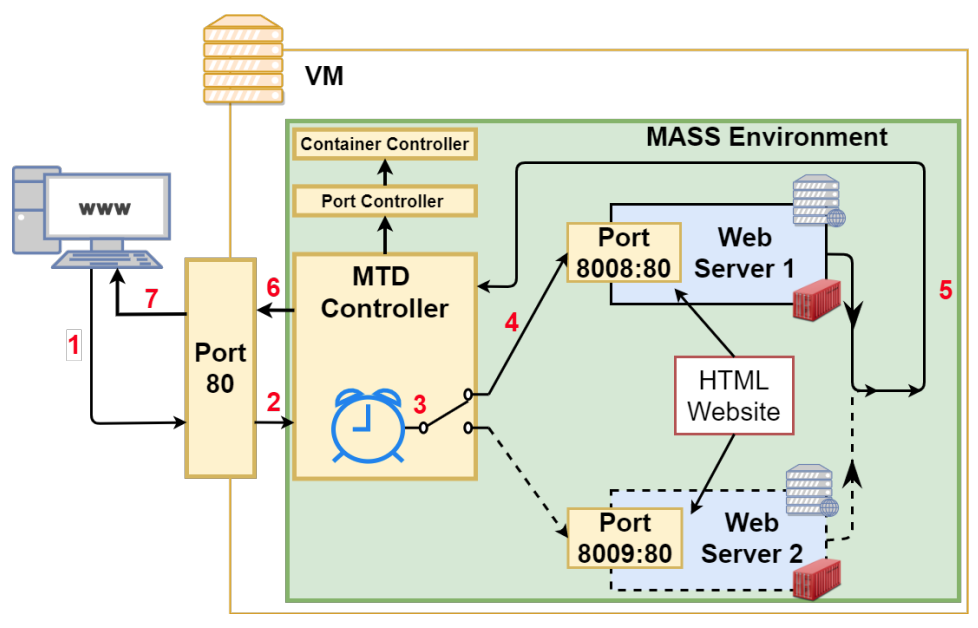
\includegraphics[width=\linewidth]{./imagenes/mass-structure.png}
    \caption{Estructura original del MASS con flujo de tráfico.\cite{MTD-DARE-DIM-MASS}}
\end{figure}

\begin{itemize}
    \item \textbf{Controlador del MTD}: Responsable de gestionar el tiempo y activar el cambio de servidor. Es capaz de realizar rotaciones tanto en intervalos fijos como dentro de un rango de tiempos especificado.
    \item \textbf{Controlador de contenedores}: Encargado de iniciar y detener los contenedores que alojan los servidores, gestionando su ciclo de vida.
    \item \textbf{Controlador de puertos}: Administra el \textit{firewall}, redirigiendo el tráfico desde el puerto 80 hacia los puertos internos del servidor activo (8008 y 8009), garantizando una correcta comunicación.
\end{itemize}

En la implementación realizada se han separado el controlador de contenedores del de puertos, siendo ambos controlados directamente por el controlador del MTD. Esta representación se puede ver en el siguiente diagrama de clases.

\begin{figure}[H]
    \centering
    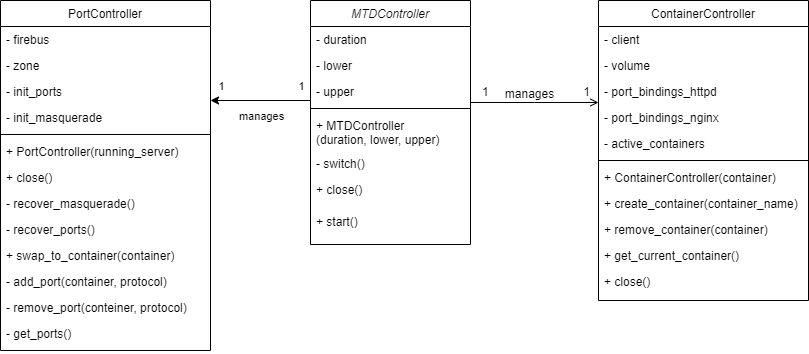
\includegraphics[width=\linewidth]{./imagenes/clases.png}
    \caption{Diagrama de clases de la implementación.}
\end{figure}

\section{Tests}
Para evaluar el comportamiento y rendimiento del MASS, se han llevado a cabo diversas pruebas, incluyendo pruebas de funcionalidad, integración, rendimiento bajo sobrecarga, uso de CPU en reposo, y pruebas de explotación.

La siguiente notación será utilizada para diferenciar los diferentes MASS evaluados:

\begin{table}[h!]
    \centering
    \begin{tabular}{|c|cc|c|}
        \hline
        \textbf{Servidor} & \multicolumn{2}{c|}{\textbf{Límite de tiempo (s)}} & \textbf{Notación} \\ 
        \cline{2-3}
        & \textbf{Lower (i)} & \textbf{Upper (j)} & \\ 
        \hline
        MTD & i & j & MTD$[i,j]$ \\ 
        MASS & 15 & 15 & MASS$[15,15]$ \\ 
        MASS & 15 & 20 & MASS$[15,20]$ \\ 
        MASS & 20 & 20 & MASS$[20,20]$ \\ 
        \hline
    \end{tabular}
    \caption{Notación para los MTD, donde se rota cada $t$ segundos, $t \in \mathbb{R}, i \leq t \leq j$.}
\end{table}

    
\subsection{Funcionalidad e integración}
Las pruebas de funcionalidad e integración se han realizado utilizando la herramienta Behave, la cual permite la ejecución de tests automatizados basados en escenarios. No se ha establecido una separación estricta entre ambos tipos de pruebas, ya que los controladores tanto de los puertos como de los contenedores emplean sus respectivos clientes para comunicarse con Docker y Firewalld, lo que implica un proceso de integración inherente en las pruebas funcionales.

Adicionalmente, se ha implementado Codecov para generar un informe sobre la cobertura del código, lo que facilita la identificación de las partes del sistema que han sido sometidas a pruebas y el porcentaje de cobertura alcanzado. Esto nos permite garantizar un nivel mínimo de calidad y robustez en el código.

\begin{figure}[h]
    \centering
    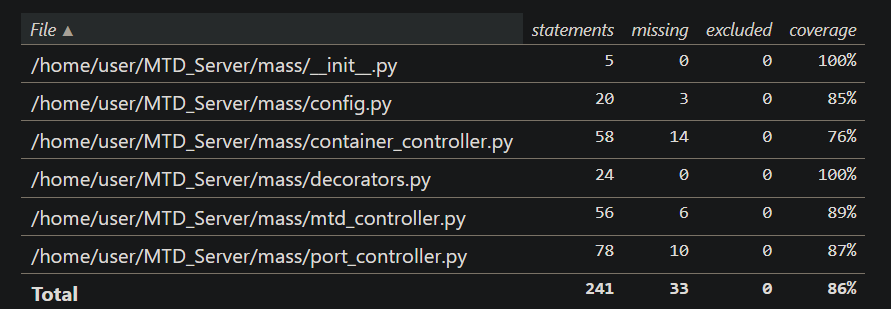
\includegraphics[width=\linewidth]{./imagenes/coverage.png}
    \caption{Cobertura del código}
\end{figure}

\subsection{Capacidad procesamiento de las peticiones}
Para medir la capacidad del MTD bajo carga, se ha utilizado Apache Benchmark desde una máquina externa. Mediante esta herramienta, se ha realizado una prueba de estrés al módulo, permitiendo observar su comportamiento y capacidad de respuesta ante un elevado número de peticiones simultáneas.

Sometiendo los diferentes servidores a un test con una concurrencia de 100 y 150,000 peticiones en total, se ha observado lo siguiente:

\begin{figure}[h]
    \centering
    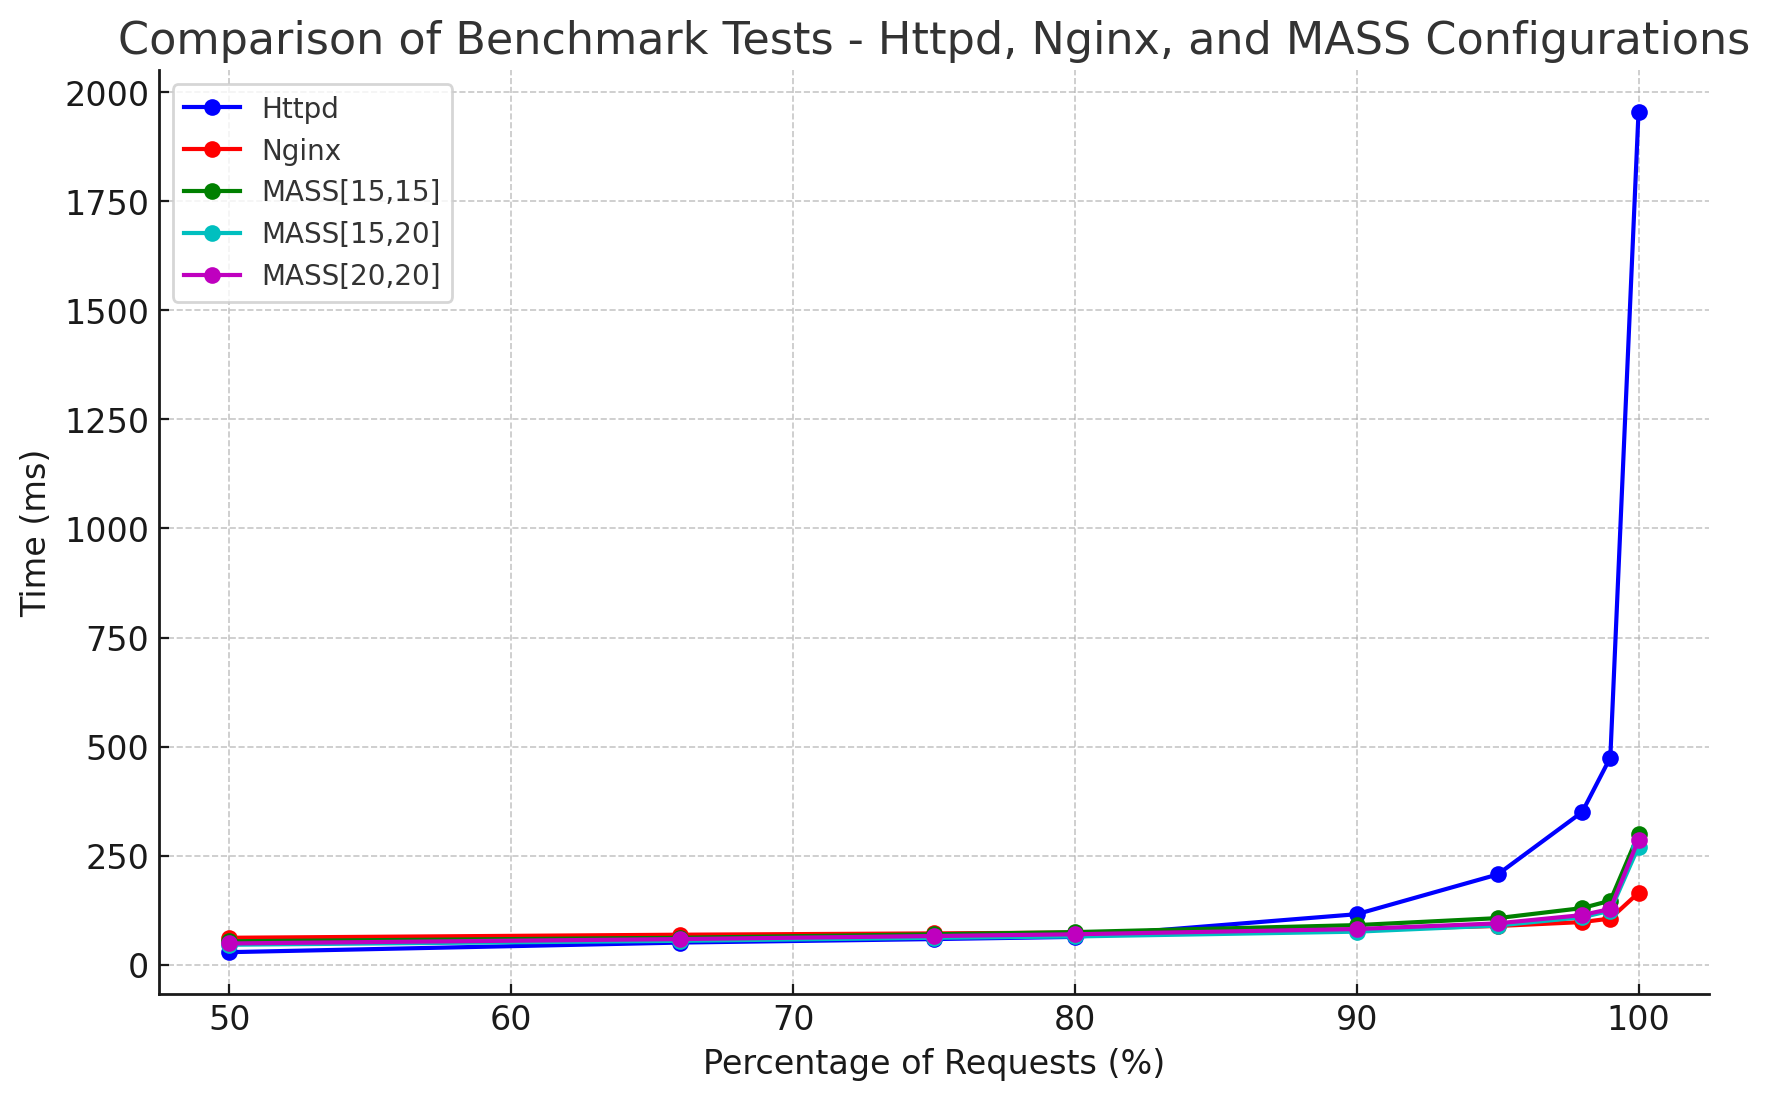
\includegraphics[width=\linewidth]{./imagenes/comparison.png}
    \caption{Comparación de percentiles de tiempo de respuesta a las peticiones}
\end{figure}

Como se puede apreciar en la figura anterior, se comparan los tiempos de respuesta de los diferentes servidores para diferentes percentiles. En todos los casos, se utilizó una concurrencia de 100 conexiones simultáneas y un total de 150,000 solicitudes realizadas.

Cabe destacar que no se ha perdido ni una petición de las realizadas, lo que indica que el rendimiento de los servidores bajo estas condiciones de prueba ha sido confiable en cuanto a la entrega de todas las solicitudes sin errores.


\subsection{Rendimiento en reposo}
Se ha evaluado el rendimiento del sistema en reposo sin ninguna interacción del usuario. Para esta evaluación, se ha empleado la herramienta sar\cite{sar}, la cual permite monitorizar el uso de recursos del sistema, en un entorno sin carga activa.

\begin{table}[H]
    \centering
    \begin{tabular}{|c|c|c|}
        \hline
        \textbf{Imagen} & \textbf{Promedio de Uso de CPU (\%)} & \textbf{Desviación Estándar (\%)} \\ 
        \hline
        Nginx & 2.18 & 1.76 \\ 
        Httpd & 2.19 & 2.0 \\ 
        MASS$[15,15]$ & 7.86 & 13.11 \\ 
        MASS$[15,20]$ & 7.82 & 12.78 \\ 
        MASS$[20,20]$ & 7.42 & 12.55 \\ 
        \hline
    \end{tabular}
    \caption{Comparativa del uso de CPU en reposo}
    \end{table}

    \begin{figure}[H]
        \centering
        \begin{subfigure}[b]{0.45\textwidth}
            \centering
            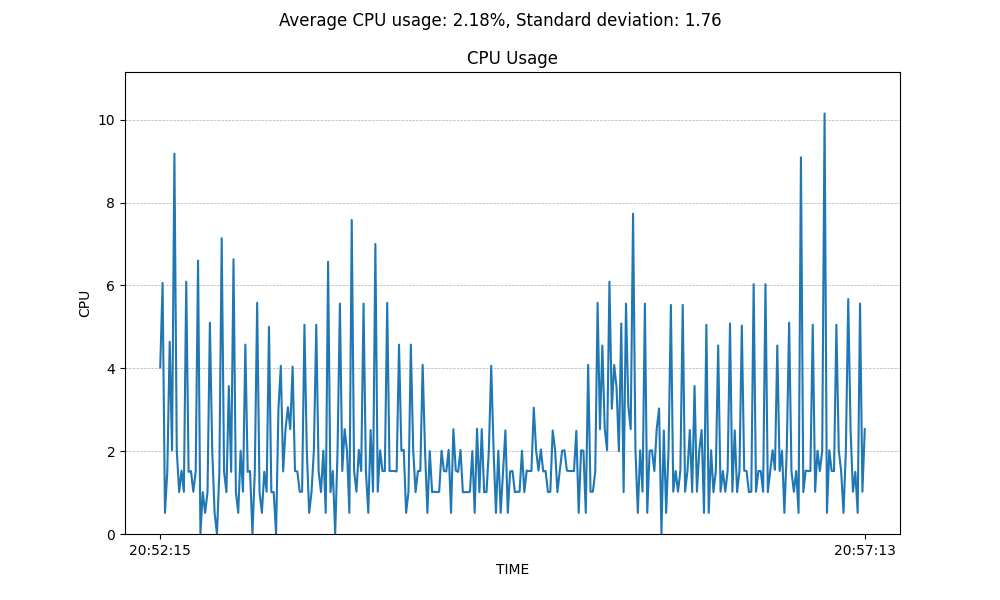
\includegraphics[width=\textwidth]{./imagenes/nginx.csv.png}
            \caption{Uso de CPU Nginx}
            \label{fig:imagen1}
        \end{subfigure}
        \hfill
        \begin{subfigure}[b]{0.45\textwidth}
            \centering
            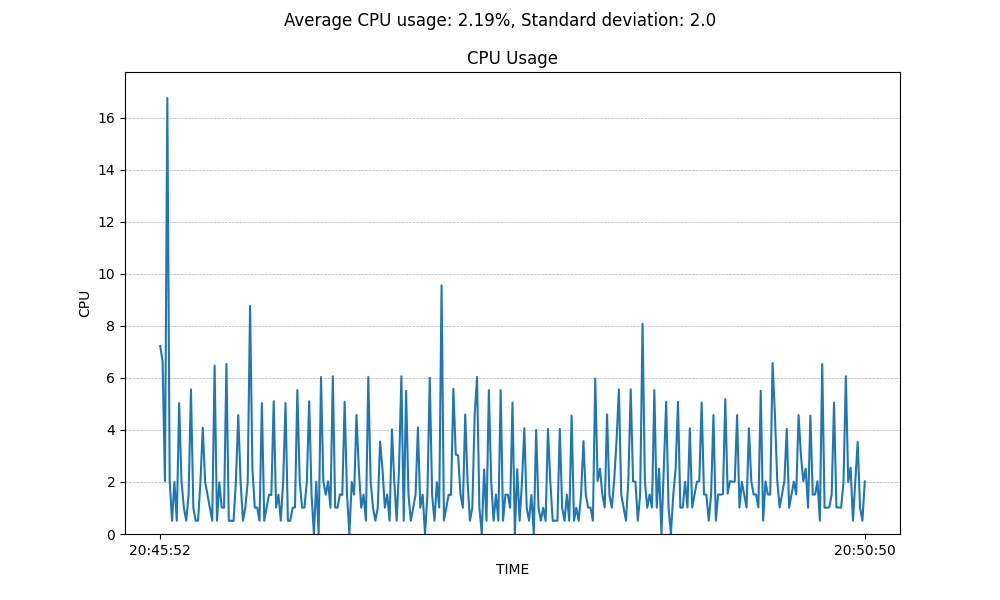
\includegraphics[width=\textwidth]{./imagenes/httpd.csv.png} 
            \caption{Uso de CPU Httpd}
            \label{fig:imagen2}
        \end{subfigure}
        
        \vspace{0.5cm} 
        
        \begin{subfigure}[b]{0.45\textwidth}
            \centering
            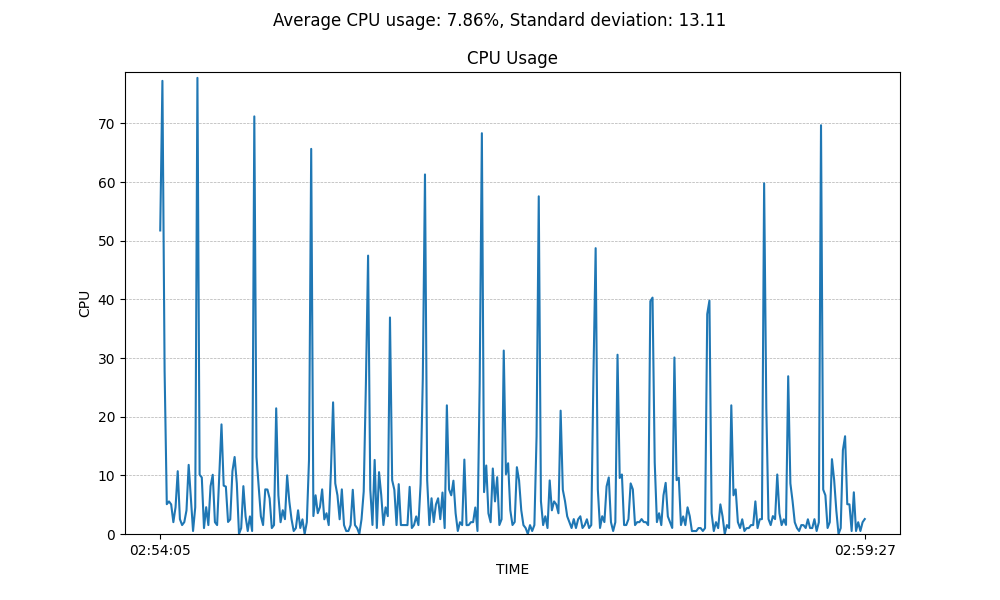
\includegraphics[width=\textwidth]{./imagenes/mtd-no-petition_u15_l15.csv.png}  
            \caption{Uso de CPU MASS$[15,15]$}
            \label{fig:imagen3}
        \end{subfigure}
        \hfill
        \begin{subfigure}[b]{0.45\textwidth}
            \centering
            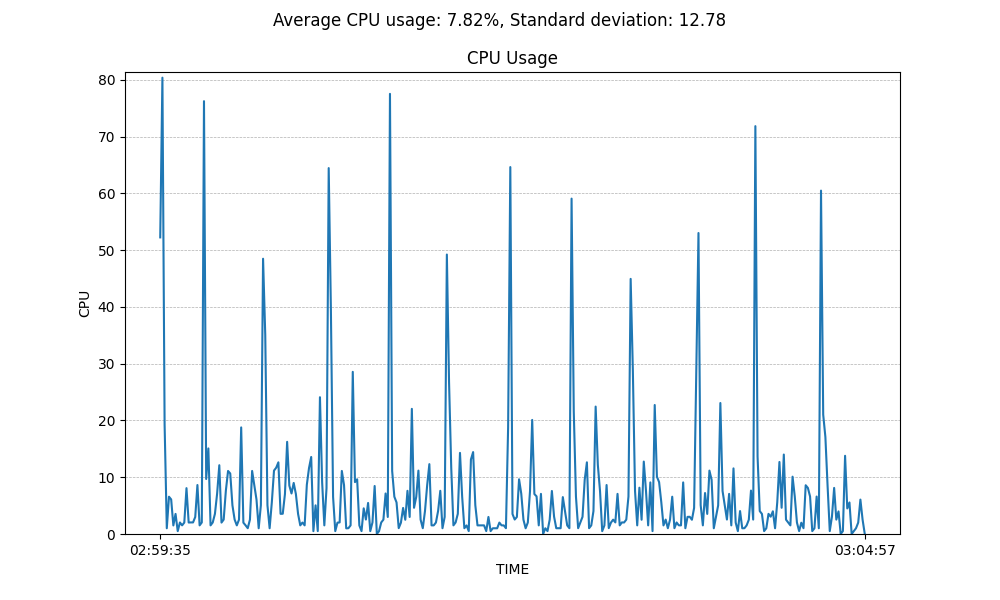
\includegraphics[width=\textwidth]{./imagenes/mtd-no-petition_u20_l15.csv.png} 
            \caption{Uso de CPU MASS$[15,20]$}
            \label{fig:imagen4}
        \end{subfigure}

        \vspace{0.5cm} 

        \begin{subfigure}[H]{0.45\textwidth}
            \centering
            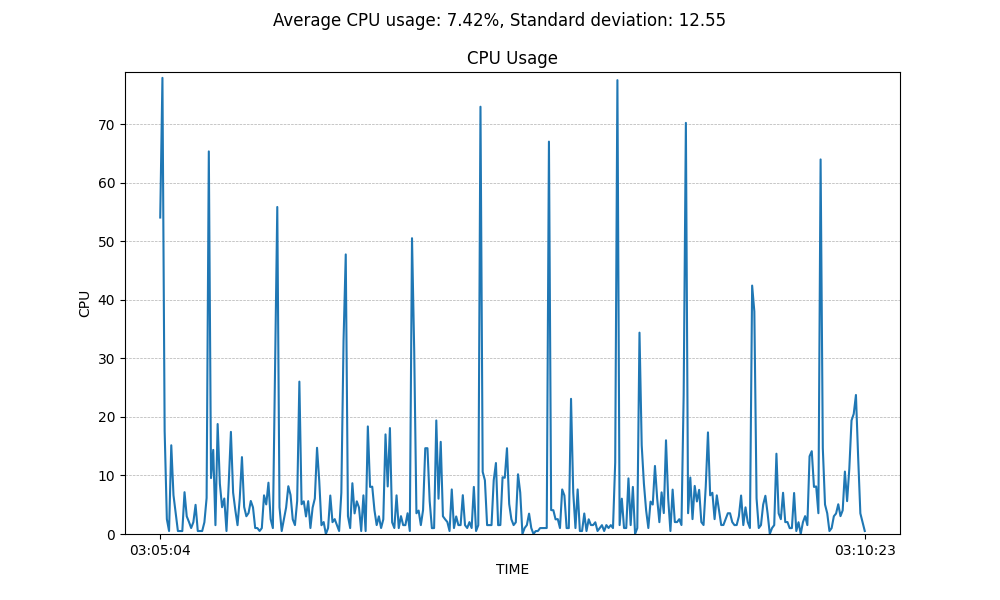
\includegraphics[width=\textwidth]{./imagenes/mtd-no-petition_u20_l20.csv.png} 
            \caption{Uso de CPU MASS$[20,20]$}
            \label{fig:imagen5}
        \end{subfigure}
        \caption{Gráficas con el uso de CPU en diferentes servidores}
    \end{figure}
    
    

\subsection{Pruebas de explotación}
Entre las pruebas realizadas, se ha incluido la explotación de la vulnerabilidad CVE-2021-41773, descubierta en versiones anteriores del servidor web Apache HTTP. Esta vulnerabilidad, que afecta a Apache 2.4.49 y 2.4.50, permite a un atacante no autenticado realizar un \textit{path traversal} para acceder a archivos fuera de los directorios permitidos. En casos más graves, la explotación de esta vulnerabilidad puede conducir a la ejecución remota de código (RCE), lo que da al atacante control sobre el sistema afectado. Para más información sobre esta vulnerabilidad, se ha utilizado el análisis detallado disponible en el blog de HackTheBox\cite{cve-2021-41773}.

El ataque se realizó desde una máquina externa, enviando solicitudes HTTP con el fin de explotar la vulnerabilidad. Estas peticiones contenían rutas que intentaban ejecutar comandos arbitrarios. Para verificar si el ataque era exitoso y si se había logrado la ejecución remota de código, se utilizó una técnica de escucha en la VM donde está alojado el contenedor.

Específicamente, la petición HTTP inyecta una petición con \cite{netcat} para enviar una traza o señal al localhost, donde había un puerto habilitado herramienta Netcat (nc) en modo escucha. Netcat fue utilizado para recibir la conexión entrante como prueba de que el servidor había ejecutado el comando enviado desde la máquina externa.

\begin{table}[H]
    \centering
    \begin{tabular}{|c|c|c|}
        \hline
        \textbf{Servidor} & \textbf{Ataques exitosos \%} \\ 
        \hline
        Nginx & - \\ 
        Httpd & 100 \\ 
        MASS$[15,15]$ & 46 \\ 
        MASS$[15,20]$ & 47.2 \\ 
        MASS$[20,20]$ & 44.4 \\ 
        \hline
    \end{tabular}
    \caption{Comparativa del número de ataques exitosos}
    \end{table}
